\PassOptionsToPackage{usenames,dvipsnames}{xcolor}
\documentclass[xelatex,aspectratio=169]{beamer}

\usepackage{xifthen,multicol,textcomp,graphicx,minted,cancel}
\usepackage{tikz,amsmath,xparse,xmpp}
\usepackage[printwatermark]{xwatermark}
\usepackage{fontspec}
\usetikzlibrary{arrows,decorations.pathreplacing}
\newcommand*{\tikzmark}[1]{\tikz[overlay, remember picture] \coordinate ({#1});}

\newcommand\blfootnote[1]{%
	\begingroup
	\renewcommand\thefootnote{}\footnote{#1}%
	% \addtocounter{footnote}{-1}%
	\endgroup
}

\usetheme{Atlassian}
\usecolortheme{whale}
\beamertemplatenavigationsymbolsempty

\title[]{Go}
\subtitle{(get happy)}
\author[]{%
	Sam Whited\\*%
	{\tiny\texttt{\href{xmpp:sam@samwhited.com}{sam@samwhited.com}}}%
}
% \date{2015--12--18}
\titlegraphic{%
	
\includegraphics[width=20mm]{images/hipchat.png}%
	\hspace*{.25\textwidth}%
	
\includegraphics[width=20mm]{images/atlassian.png}%
}

% Define a font family that supports IPA characters.
\usefonttheme{professionalfonts}
\usefonttheme{serif}
\newfontfamily\ipa{Charis SIL}
\newfontfamily\apl{APL385 Unicode}
\newfontfamily\calluna{Calluna}
\newfontfamily\callunasans{Calluna Sans}
% \newfontfamily\geotica{Geotica Three}
% \setmainfont{Circular Pro}
\setmainfont{Calluna Sans}
\newfontfamily\dejavusansmono{DejaVu Sans Mono}
% \setmonofont{DejaVu Sans Mono}
\setmonofont{Source Code Pro}
\defaultfontfeatures{Ligatures=Common, Mapping=tex-text}
\newfontfamily\useligatures[Mapping=tex-text, Ligatures={Common, Rare}]{Calluna}

% \usepackage{newunicodechar}
% \newfontfamily{\Carrows}{TeX Gyre Adventor}
% \newunicodechar{↑}{\arrowresize{\Carrows ↑}}
% \newcommand{\arrowresize}[1]{%
% 	\sbox0{\ttfamily │}%
% 	\setlength{\dimen8}{\dimexpr\ht0+\dp0\relax}%
% 	\makebox[\wd0]{\raisebox{-.5\dp0}[\ht0][\dp0]{\resizebox{\width}{.8\dimen8}{#1}}}%
% }

\NewDocumentEnvironment{fancyquote}{o}{%
	\begin{centering}
		\Huge„\Large\calluna\itshape
}{%
	\Huge“\Large
		\begin{flushright}
			\IfNoValueTF{#1}{}{\normalfont---\callunasans#1}
		\end{flushright}
	\end{centering}
}

\newsavebox\mybox
\savebox\mybox{\tikz[color=CheetoOrange,opacity=0.3]\node{CAUTION};}
\newwatermark*[
	pages=2,
	angle=0,
	scale=6,
	xpos=25,
	ypos=51
]{\usebox\mybox}


\begin{document}

\begin{frame}
	\maketitle
\end{frame}

\begin{frame}
	\begin{flushleft}
		{\LARGE Gophers at work.}
	\end{flushleft}
	\begin{flushleft}
		These slides explain why I think Go is a good fit for HipChat (and
		Bitbucket, and anything else in the cloud\ldots\ and a lot of other stuff
		not in the cloud). They are not an introduction to Go. Most of them were
		cribbed from Rob Pike, Andrew Gerrand, and others. The Gopher logo is by
		Renee French.
	\end{flushleft}
	\begin{tikzpicture}[remember picture,overlay]
		\node [xshift=-0.25\textwidth,yshift=6em] at (current page.south east)
		{
\includegraphics[width=7em]{images/gopherhorse.png}};
	\end{tikzpicture}
\end{frame}

\begin{frame}
	\only<1>{\frametitle{The Zen of Python}}
	\only<2->{\frametitle{The Zen of \xcancel{Python} Go}}
	\begin{tikzpicture}[remember picture,overlay]
		\node [xshift=-0.25\textwidth,yshift=-10em] at (current page.north east)
		{%
			\only<1>{
\includegraphics[width=7em]{images/python.png}}%
			\only<2->{
\includegraphics[width=7em]{images/flyinggopher.jpg}}%
		};
	\end{tikzpicture}
	\tiny
	% \defbeamertemplate{itemize item}{circle}{\tiny\raise0.5pt\hbox{\textbullet}}
	\setbeamertemplate{itemize item}{\tiny\raisebox{0.1em}{\textbullet}}
	\begin{itemize}
		\item Beautiful is better than ugly.
		\item Explicit is better than implicit.
		\item Simple is better than complex.
		\item Complex is better than complicated.
		\item Flat is better than nested.
		\item Sparse is better than dense.
		\item \only<1-2>{Readability counts.}\only<3>{{\small Readability counts.}}
		\item Special cases aren't special enough to break the rules.
		\item Although practicality beats purity.
		\item Errors should never pass silently.
		\item Unless explicitly silenced.
		\item In the face of ambiguity, refuse the temptation to guess.
		\item There should be one---and preferably only one---obvious way to do it.
		\item Although that way may not be obvious at first unless you're \only<1>{Dutch}\only<2->{\cancel{Dutch} Rob Pike}.
		\item Now is better than never.
		\item Although never is often better than \emph{right} now.
		\item If the implementation is hard to explain, it's a bad idea.
		\item If the implementation is easy to explain, it may be a good idea.
		\item Namespaces are one honking great idea --- let's do more of those!
	\end{itemize}
	\blfootnote{http://talks.golang.org/2012/zen.slide}
\end{frame}

\begin{frame}
	\frametitle{The Zen of Go}
	\only<1>{\setbeamercolor{item}{fg=Violet}}
	\only<2>{\setbeamercolor{item}{fg=CheetoOrange}}
	\only<3>{\setbeamercolor{item}{fg=Mauve}}
	\only<4>{\setbeamercolor{item}{fg=Slate}}
	\only<5-6>{\setbeamercolor{item}{fg=LimeGreen}}
	\only<7>{\setbeamercolor{item}{fg=Brown}}
	\only<8>{\setbeamercolor{item}{fg=BrightPink}}
	\only<9>{\setbeamercolor{item}{fg=Cyan}}
	\begin{enumerate}
		\item<1> Familiarity admits brevity
		\item<2> Dependency analysis should be easy
		\item<3> Composition is better than inheritance
		\item<4> Static linking is better than dynamic linking
		\item<5-6> If it's worth complaining about, it's worth fixing
		\item<6> If it's not worth fixing, it's not worth mentioning
		\item<7> Long term clarity is better than short term convenience
		\item<8> Semicolons are for parsers, not for people
		\item<9> Don't communicate by sharing memory, share memory by communicating
	\end{enumerate}
	\vspace*{\fill}\hspace*{0.75\textwidth}
	\vspace*{-4em}
	\begin{tikzpicture}[remember picture,overlay]
		\only<1-8>{
		\node [xshift=-0.25\textwidth,yshift=2.5em] at (current page.south east)
		{
\includegraphics[width=20mm]{images/gopher.png}};}
		\only<9>{
		\node [xshift=-0.25\textwidth,yshift=1.5em] at (current page.south east)
		{
\includegraphics[width=20mm]{images/gopher.png}};}
	\end{tikzpicture}
\end{frame}

\begin{frame}
\def\firstcircle{(0,0) circle (2cm)}
\def\secondcircle{(60:2.5cm) circle (2cm)}
\def\thirdcircle{(0:2.5cm) circle (2cm)}
\begin{figure}[!h]
\centering
\begin{tikzpicture}
	\begin{scope}[shift={(3cm,-5cm)}, fill opacity=0.5]
		\fill[red] \firstcircle;
		\fill[green] \secondcircle;
		\fill[blue] \thirdcircle;
		\draw \firstcircle node[below] {Ease\hspace*{2em}};
		\draw \secondcircle node [above] {Compile time};
		\draw \thirdcircle node [below] {\hspace*{2em}Speed};
	\end{scope}
	\begin{scope}[shift={(3cm,-5cm)}]
		\node [anchor=center] at (1em, 3em)
		{
\includegraphics[width=1.5em]{images/python.png}};
		\node [anchor=center] at (6em, 3em)
		{
\includegraphics[width=1.5em]{images/c.png}};
		\node [anchor=center] at (3.25em, -1em)
		{
\includegraphics[width=1.5em]{images/rust.png}};
		\node [anchor=center] at (3.25em, 2em)
		{
\includegraphics[width=2em]{images/golang.png}};
		% \node [anchor=center] at (999em, 999em)
		% {
\includegraphics[width=1.5em]{images/perl.png}};
	\end{scope}
\end{tikzpicture}
\end{figure}
\end{frame}

\begin{frame}
	\begin{flushleft}
	ECMAScript 6, Python 3, Java 8, C++14, etc. compete by adding
	\only<1>{features}\only<2->{\cancel{features} complexity}.
	\end{flushleft}

	\begin{flushleft}
		\only<3->{As of Go 1.0: the language is done.}
		\only<4->{Finished.}
		\only<5->{Complete.}
	\end{flushleft}
	\begin{flushleft}
		\vspace*{\fill}
		\only<6->{{\Large This is a feature.}}
		\vspace*{\fill}
	\end{flushleft}
\end{frame}

\begin{frame}
	\frametitle{The Prime Directive}
	\begin{flushleft}
		Go \emph{must} remain simple.
	\end{flushleft}
	\begin{tikzpicture}[remember picture,overlay]
		\node [xshift=-0.25\textwidth,yshift=6em] at (current page.south east)
		{
\includegraphics[width=7em]{images/gala.jpg}};
	\end{tikzpicture}
\end{frame}

{
\renewcommand{\fcolorbox}[4][]{#4}
\begin{frame}[fragile]
	\frametitle{Methods}
\begin{minted}{go}
func (u GeoURI) Location() (float64, float64, error)
\end{minted}
\end{frame}

\begin{frame}[fragile]
	\frametitle{Simple is better than complex}
\begin{minted}{go}
type GeoURI string
func (u GeoURI) Location() (float64, float64, error) {…}
\end{minted}
\begin{itemize}[<+(1)->]
	\item Methods \emph{are} functions
	\item Receiver is just an argument (like Python), no `this' or other magic
\end{itemize}
\end{frame}
\begin{frame}[fragile]
	\frametitle{Simple is better than complex}
\begin{minted}{go}
type GeoURI string
func (GeoURI) Location() (float64, float64, error) {…}
\end{minted}
\begin{itemize}
	\item Methods \emph{are} functions
	\item Receiver is just an argument (like Python), no `this' or other magic
	\item Although the receiver can be unnamed
\end{itemize}
\end{frame}
\begin{frame}[fragile]
	\frametitle{Simple is better than complex}
\begin{minted}{go}
type GeoURI string
func (u GeoURI) Location() (float64, float64, error) {…}
\end{minted}
\begin{itemize}
	\item Methods \emph{are} functions
	\item Receiver is just an argument (like Python), no `this' or other magic
	\item Although the receiver can be unnamed
	\item Any type may have methods (struct, interface, strings, func pointers\ldots)
\end{itemize}
\end{frame}

\begin{frame}[fragile]
	\frametitle{Flat is better than nested}
\begin{minted}{go}
type GeoURI string
func (u GeoURI) Location() (float64, float64, error) {…}
\end{minted}
\begin{flushleft}
	Methods not nested in classes (not that there are any classes for them to be
	nested in)
\end{flushleft}
\end{frame}

\begin{frame}[fragile]
	\frametitle{Readability counts}
\begin{minted}{go}
func (u GeoURI) Location() (lat,long float64, err error)
\end{minted}
\begin{flushleft}
	Return types may be named, no more boolean traps (yey)!
	\only<2->{\\Also note that lat, long take the same type; let's not be redundant and repeat ourselves!}
\end{flushleft}
\only<3->{%
\begin{flushleft}
	Go is concise and expressive while maintaining readability.
\end{flushleft}
}
\end{frame}
}

\begin{frame}
	\begin{fancyquote}[Rob Pike]
	Be concise, while remaining expressive.
	\end{fancyquote}
	\begin{tikzpicture}[remember picture,overlay]
		\node [xshift=0,yshift=-5em] at (current page.center)
		{
\includegraphics[width=15em]{images/gophersimple.jpg}};
	\end{tikzpicture}
\end{frame}

\begin{frame}
	\begin{fancyquote}[Every other post on go-nuts]
		But we need <insert-feature-here> for expressiveness!
	\end{fancyquote}
\end{frame}

\begin{frame}
	\frametitle{Readability is not expressiveness (or conciceness)}
	\centerline{\apl{⊃ 1 ω ∨ . ∧ 3 4 = +/ +⌿ 1 0 ‾1 ∘.θ 1 - ‾1 Φ″ ⊂ ω}}
\end{frame}

{
\renewcommand{\fcolorbox}[4][]{#4}
\begin{frame}[fragile]
	\frametitle{Readability counts}
\begin{minted}{C}
// C
char *(*fp)( int, float *);
\end{minted}
\end{frame}
\begin{frame}[fragile]
	\frametitle{Readability counts}
	\let\thefootnote\relax
	\footnote{The Clockwise Spiral Rule; \url{http://c-faq.com/decl/spiral.anderson.html}}
	\setlength{\lineskip}{0pt}
\begin{minted}{C}
     ╭────────────────────╮
     │ ╭───╮              │
     │ │╭─╮│              │
     │ │↑ ││              │
char *(*fp)( int, float *);
 ↑   │ │  ││              │
 │   │ ╰──╯│              │
 │   ╰─────╯              │
 ╰────────────────────────╯
\end{minted}
\end{frame}
\begin{frame}
\centerline{
\includegraphics[width=0.75\textwidth]{images/jackie.jpg}}
\end{frame}
\begin{frame}[fragile]
	\frametitle{Readability counts}
\begin{minted}{go}
// Go
var fp *func(int, *float64) *byte
\end{minted}
\end{frame}
\begin{frame}[fragile]
	\frametitle{Readability counts}
	\setlength{\lineskip}{0pt}
\begin{minted}{go}
    ╭──╮ ╭──╮               ╭─╮
    ↑  │ │  │               │ ↓
var fp *func(int, *float64) *byte
       │ │  │               │
       ╰─╯  ╰───────────────╯
\end{minted}
\end{frame}
\begin{frame}[fragile]
	\frametitle{Readability counts}
\begin{minted}{C}
void (*signal(int, void (*fp)(int)))(int);
\end{minted}
\end{frame}
\begin{frame}[fragile]
	\frametitle{Readability counts}
	\setlength{\lineskip}{0pt}
\begin{minted}{C}
      ╭─────────────────────────────╮
      │                  ╭───╮      │
      │  ╭───╮           │╭─╮│      │
      │  ↑   │           │↑ ││      │
void (*signal(int, void (*fp)(int)))(int);
 ↑    │      │      ↑    │  ││      │
 │    ╰──────╯      │    ╰──╯│      │
 │                  ╰────────╯      │
 ╰──────────────────────────────────╯
\end{minted}
\end{frame}
\begin{frame}[fragile]
	\frametitle{Readability counts}
\begin{minted}{go}
var signal func(int, *func(int)) *func(int)
\end{minted}
\end{frame}
}

\begin{frame}
	\frametitle{TL;DR}
	\begin{itemize}[<+(1)->]
			\item Readable code is reliable code.
			\item It's easy to understand.
			\item It's easy to work on.
			\item It's easy to debug.
			\item It's easy to fix.
	\end{itemize}
	\begin{tikzpicture}[remember picture,overlay]
		\node [xshift=-0.40\textwidth,yshift=4em] at (current page.south east)
		{
\includegraphics[width=20em]{images/race.png}};
	\end{tikzpicture}
\end{frame}

\begin{frame}
\begin{centering}
\texttt{\tiny
─────────▄██████████████████▄─────\\
────────██▀░░░░░░░░░░░░░░░░▀██▄───\\
───────█▌░░▄░░░░░░░▀▄▄▀░░░░░░▀█───\\
──────█▌░░░▀███▄░░▀▄▄▄▄▀░░░░░░▀█──\\
─────█▌░░░░█▀──▀▄░░░░░░░░░▄▄█▀░▐█─\\
────█▌░░░░░█─────█░▄▄▄░░▄▀▀▀▀▄░░▐█\\
───█▌░░░░░░█──█──█░░░░░█─────█░░░█\\
──█▌░░░░░░░░▀▄▄▄▀░░░░░░█──█──█░░░█\\
─█▌░░░░░░░░░░░░░░▄░░▄░░░▀▄▄▄▀░░░░█\\
█▌░░░░▄▀▀▄░░░░░▀▀░░░░▀▀░░░░░░░░░░█\\
█░░░░░▀▄░░░░░░░▄▀░▀▄░░░░░▄▀▀▄░░░░█\\
█░▐░░░░░▀▀▀▀▀▀▀░░░░░▀▀▄▄▄▄▄▄▀░░▌░█\\
█░░▌▄░░░░░░▄█▀▀█▀▀█▀▄░░░░░░░▄░▐░░█\\
█░░▌█▀█▀▀█▀─█──█──█──█▀▀█▀▀██░▐░░█\\
█░▐░█▄█▄▄█▄▄█▄▄█▄▄█▄▄█▄▄█▄██░░▐░░█\\
█░░░███████████████████████░░░░▌░█\\
█░░░█▄─█──█──█──█──█──█──█▀░░░░░░█\\
█░░░░▀██▄▄█▄▄█▄▄█▄▄█▄▄█▄█▀░░░░░░▐█\\
█▌░░░░░░░░░░░░░░░░░░░░░░░░░░░░░▄█▀\\
─█▄░░░░░░░░░░░░░░░░░░░░░░░░░░░▄█──\\
──█▄░░░░░░░▀▄▄▄▄▄▄▄▀░░░░░░░░░▄█───\\
───██▄░░░░░░░░░░░░░░░░░░░░░▄██────\\
────▀██▄░░░░░░░░░░░░░░░░░▄██▀─────\\
──────▀███████████████████▀───────\\
}
\end{centering}
\centering{Go is very complex, but very good at hiding it.}
\end{frame}

\begin{frame}
	\begin{fancyquote}[Rob Pike (again)]
		Simplicity is the art of hiding complexity
	\end{fancyquote}
\end{frame}

\begin{frame}
	\begin{fancyquote}
		\useligatures{Simplicity is complicated.}
	\end{fancyquote}
	\blfootnote{http://talks.golang.org/2014/compiling.slide}
\end{frame}

\begin{frame}
	\begin{centering}
		\Large Go uses a:\\
		\vspace*{1em}
		\small hybrid stop-the-world/concurrent, non-generational, non-compacting,
		fully precise, tri-color, mark-and-sweep, sub 10ms latency, garbage
		collector.\\
	\end{centering}
	\only<2>{%
	\vspace*{1em}
	\begin{centering}
		And you never have to think about it or see it.\\
	\end{centering}
	}
\end{frame}

\begin{frame}
	\centerline{
\includegraphics[width=0.75\textwidth]{images/nofree.jpg}}
\end{frame}

\begin{frame}[fragile]
	\frametitle{Example \lmss{№} 1}
\begin{minted}{go}
package main

import (
  "fmt"
)

func main() {
  fmt.Println("Hello Wörld")
}
\end{minted}
\end{frame}

\begin{frame}[fragile]
	\frametitle{Example \lmss{№} 2}
\begin{minted}{go}
import ( "fmt"; "log"; "net/http" )

func многоGophers(w http.ResponseWriter, req *http.Request) {
  fmt.Fprintf(w, "много Gophers!\n")
}

func main() {
  http.HandleFunc("/", многоGophers)
  err := http.ListenAndServe("localhost:12345", nil)
  if err != nil {
    log.Fatal("ListenAndServe: ", err)
  }
}
\end{minted}
\end{frame}

\section[]{Concurrency}
\frame{\sectionpage}

\let\thefootnote\relax

\begin{frame}
	\frametitle{Concurrency}
	\begin{flushleft}
		Like Erlang and friends, Go's concurrency model is based on CSP.
		\footnote{C. A. R. Hoare: Communicating Sequential Processes (CACM 1978)}
	\begin{tikzpicture}[remember picture,overlay]
		\node [xshift=0,yshift=-4em] at (current page.center)
		{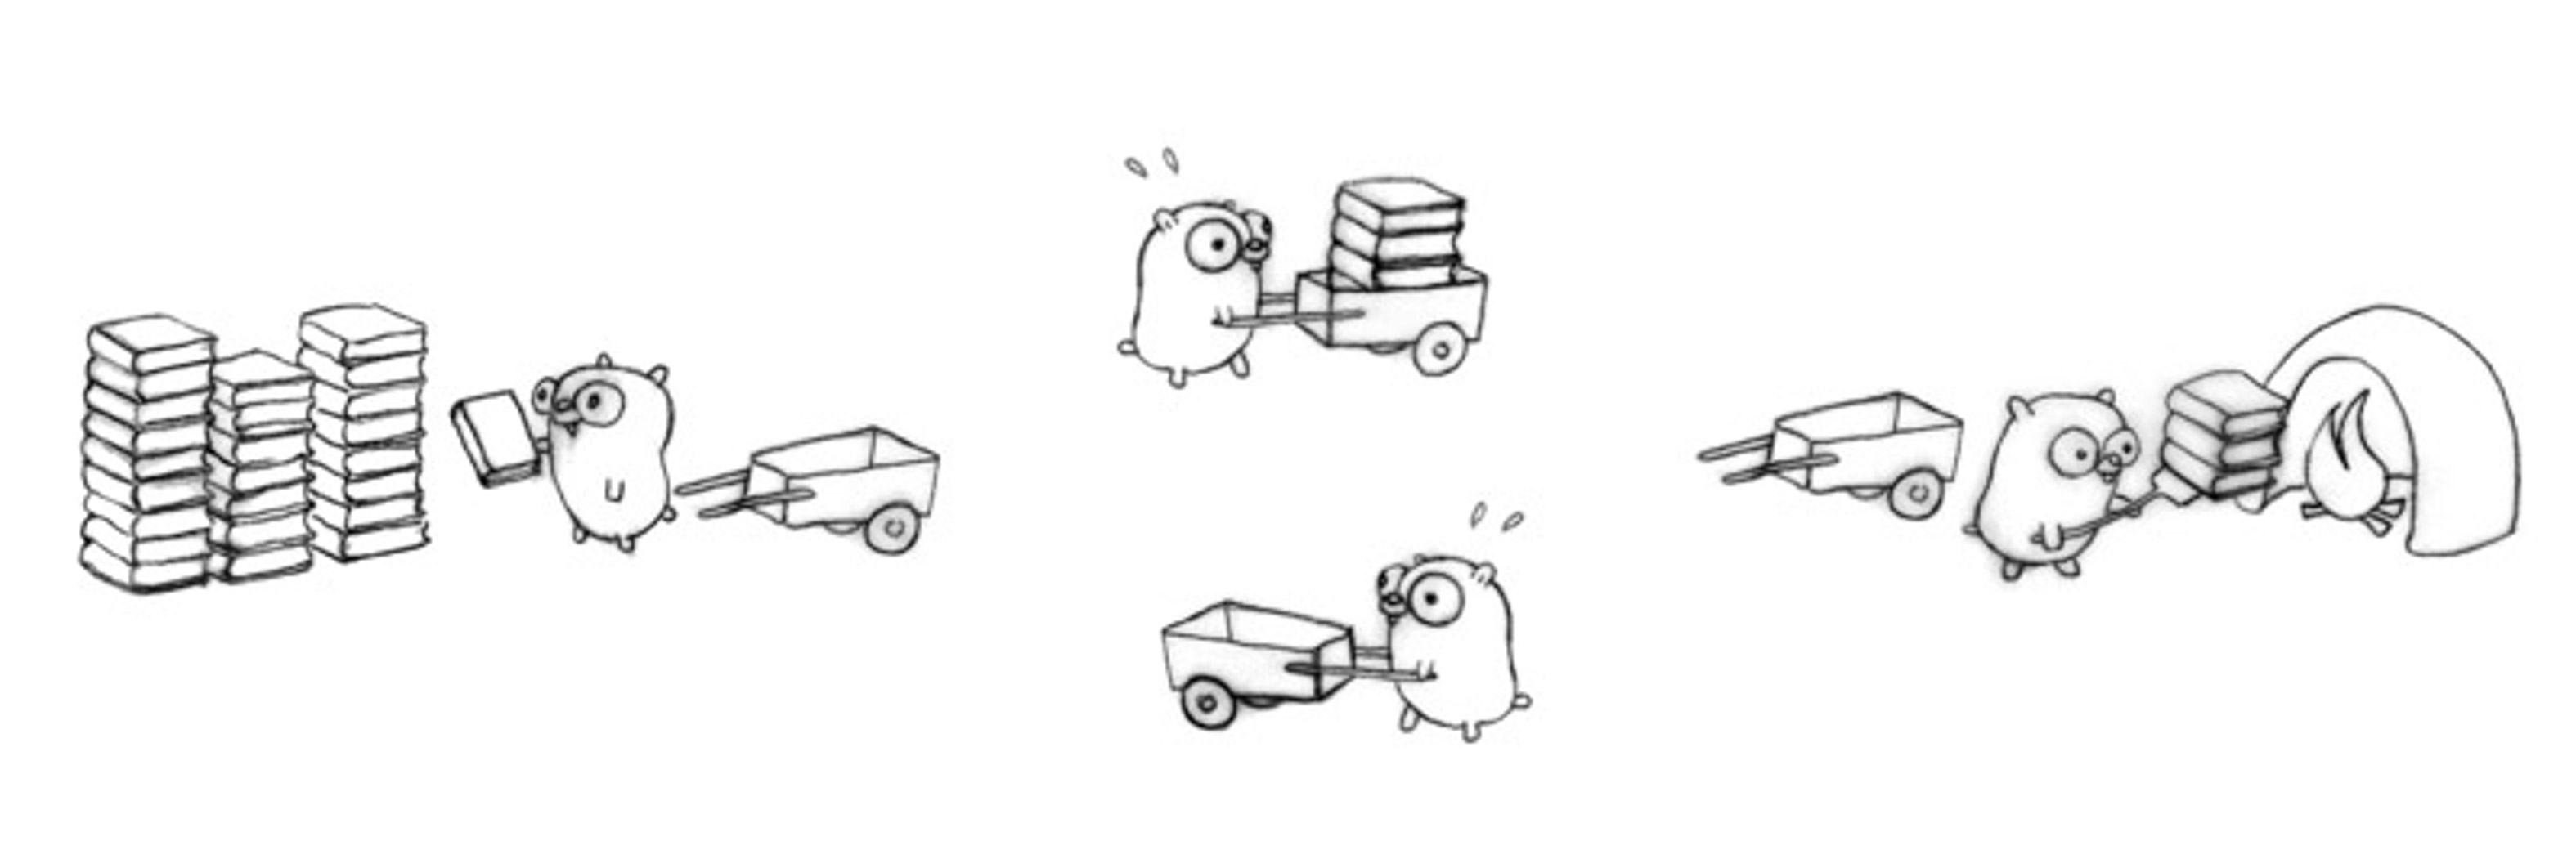
\includegraphics{images/gophercomplex1.jpg}};
	\end{tikzpicture}
	\end{flushleft}
\end{frame}

\begin{frame}
	\frametitle{Parallelism is now easy}
	\centerline{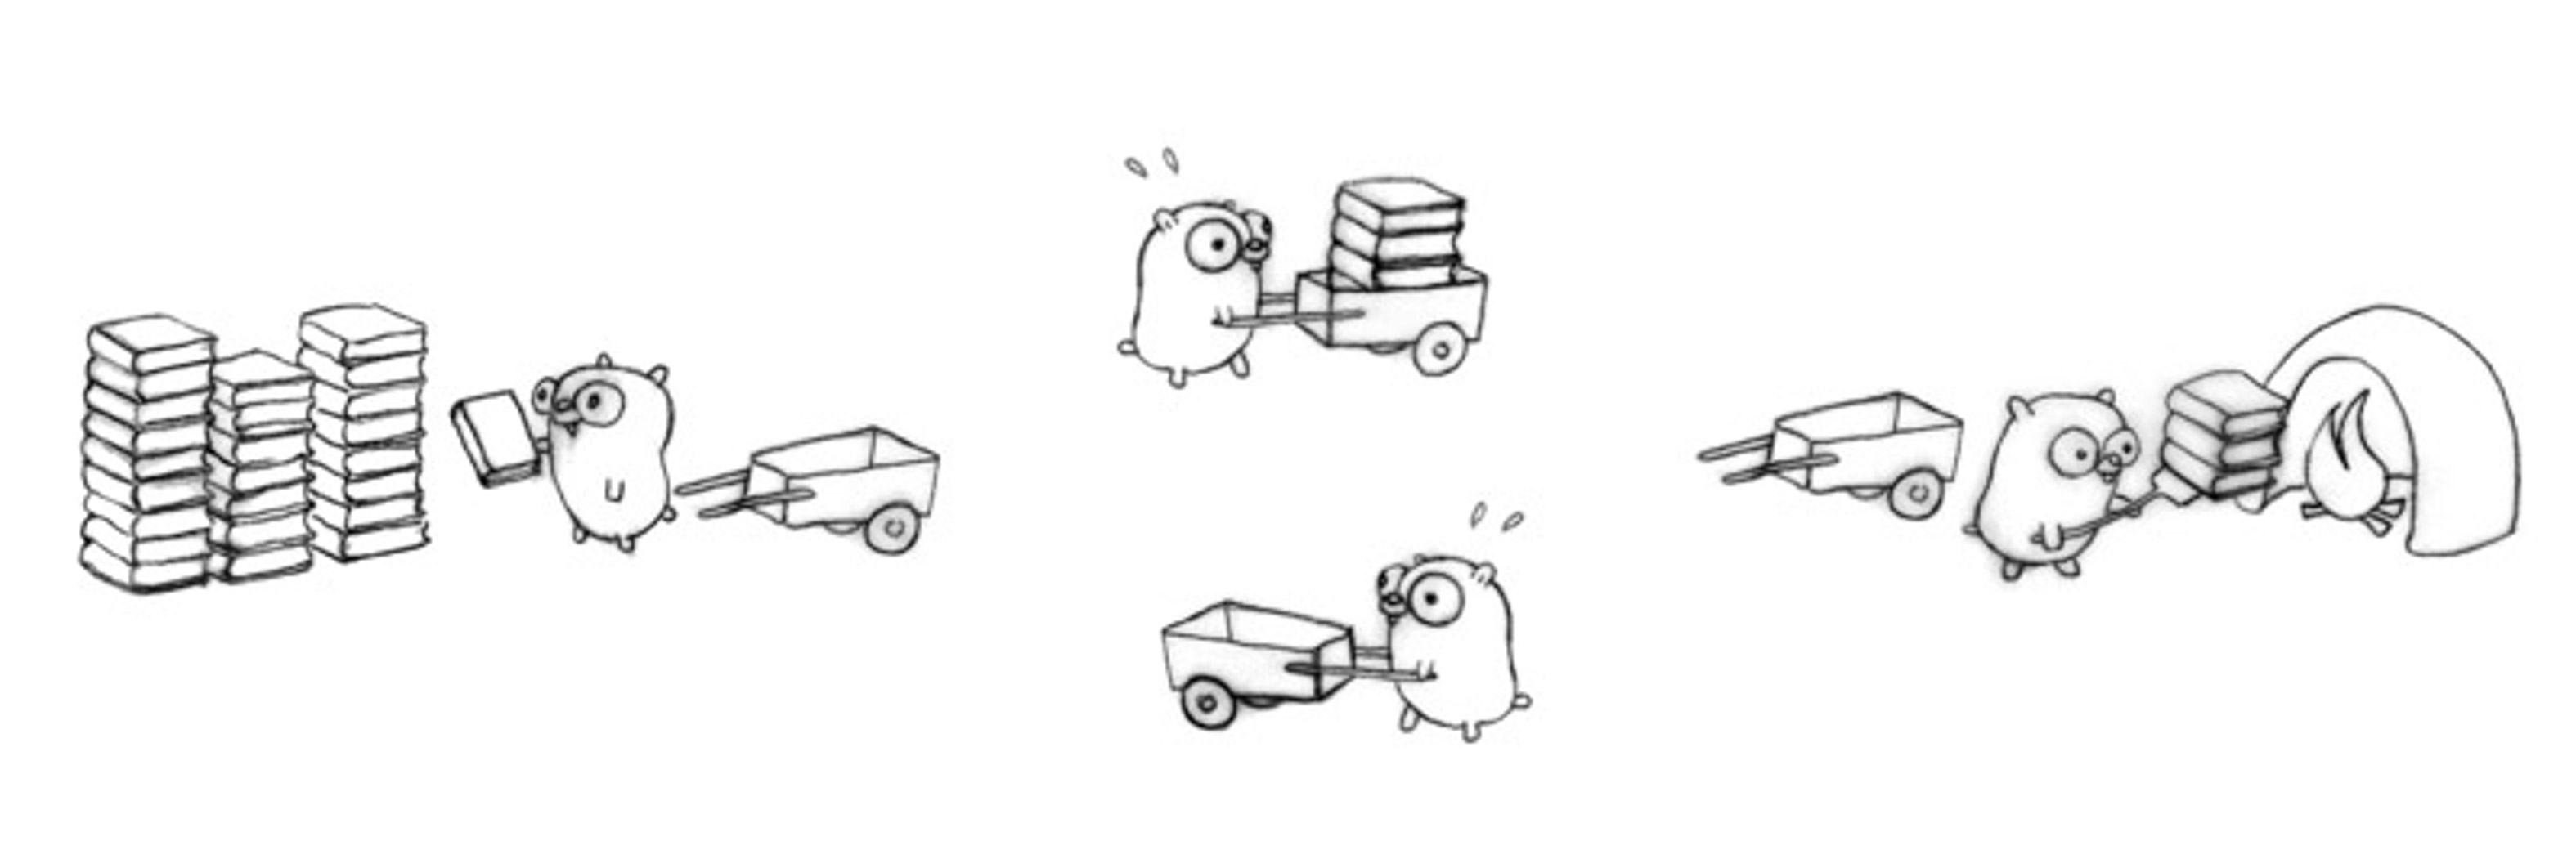
\includegraphics{images/gophercomplex1.jpg}}
	\centerline{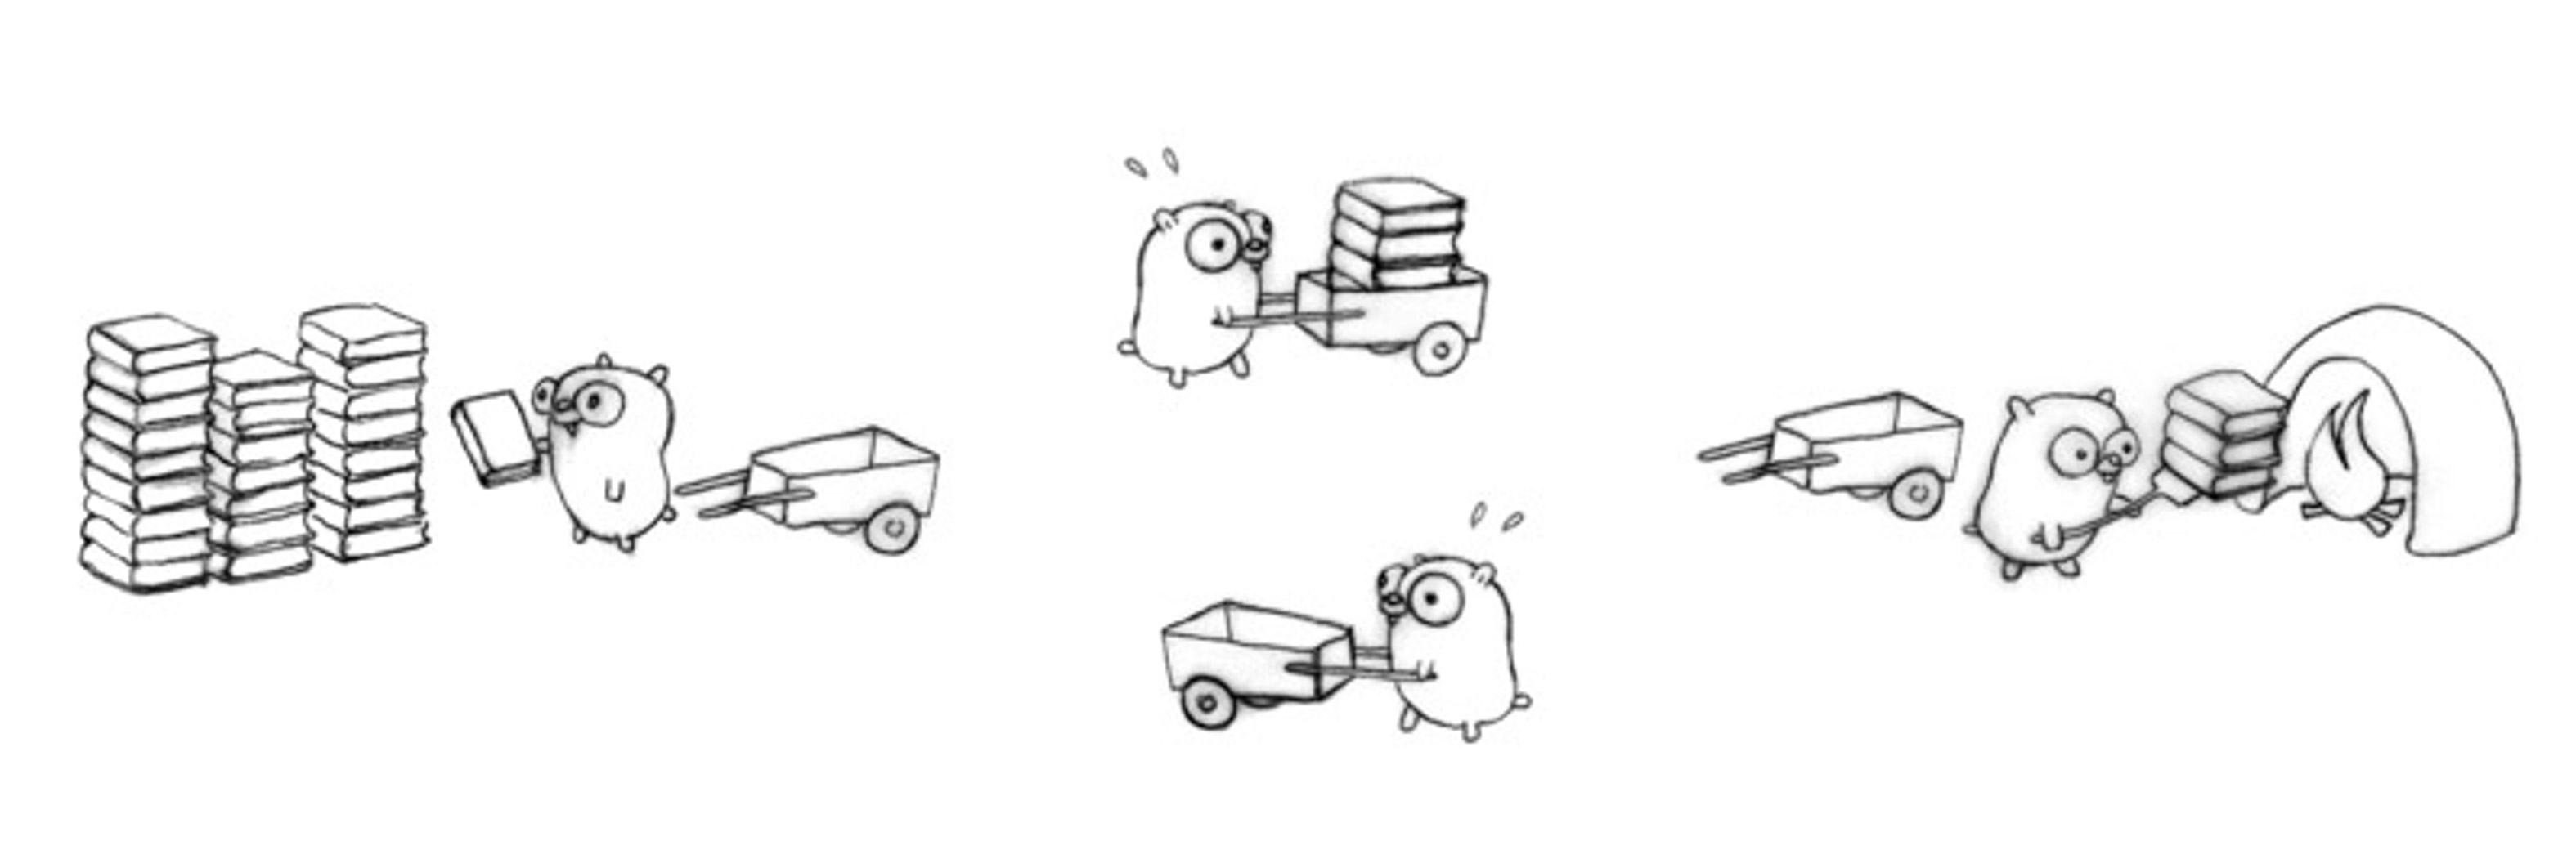
\includegraphics{images/gophercomplex1.jpg}}
\end{frame}

\begin{frame}[fragile]
	\frametitle{Go Routines}
\begin{minted}{go}
go func() {
  select { } // Block forever
}()
println("A useless goroutine")
\end{minted}
\begin{flushleft}
	Like using `\&' to background a process in Unix.
\end{flushleft}
\end{frame}

\begin{frame}
	\frametitle{Go Routines}
	\only<1>{\setbeamercolor{item}{fg=BrightPink}}
	\only<2>{\setbeamercolor{item}{fg=LimeGreen}}
	\only<3>{\setbeamercolor{item}{fg=CheetoOrange}}
	\begin{enumerate}
		\item<1> Goroutines are cheap (overhead limited to stack frame allocation)
		\item<2> Multiplexed onto threads as necessary
		\item<3> Goroutines do not block other goroutines
	\end{enumerate}
\end{frame}

\begin{frame}[fragile]
	\frametitle{Communication}
\begin{minted}{go}
c  := make(chan int)    // Unbuffered channel of ints
bc := make(chan int, 2) // Buffered channel of ints (size 2)

<-c   // Blocks until something is pushed to C
bc<-1 // Push to bc
bc<-2 // Push to bc (buffer is now full)
bc<-3 // Blocks until something is popped from bc
\end{minted}
\begin{flushleft}
	Like pipes in Unix, except channels are unbuffered by default.
\end{flushleft}
\end{frame}

\begin{frame}[fragile]
	\frametitle{Who needs Generators?}
	Use unbuffered channels.
\tiny
\begin{minted}[frame=single]{go}
func fib(n int) chan int {
  c := make(chan int)
  go func() {
    a, b := 0, 1
    for i := 0; i < n; i++ {
      a, b = b, a+b
      c <- a
    }
    close(c)
  }()
  return c
}

func main() {
  for x := range fib(10){
    fmt.Println(x)
  }
}
\end{minted}
\note{Channels are also first class values (they can be sent over channels).}
\end{frame}

\begin{frame}[fragile]
	\frametitle{Who needs semaphores?}
	Use buffered channels.
\tiny
\begin{minted}[frame=single]{go}
var sem = make(chan int, MaxRequests)

func Serve(queue chan *Request) {
  for req := range queue {
    req := req // Copy and shadow req; legal and idiomatic.
    sem <- 1   // Will block after the buffer is full
    go func() {
      process(req)
      <-sem
    }()
  }
}
\end{minted}
\end{frame}

\begin{frame}
	Go is a bit like Python:
	\begin{itemize}
			\item Simple
			\item Flexible
			\item Fun
	\end{itemize}
	But it's a bit different too:
	\begin{itemize}
			\item Fast
			\item Concurrent
			\item Sanely typed
	\end{itemize}
\end{frame}


\section[]{Tooling}
\frame{\sectionpage}

\begin{frame}
	\begin{flushleft}
		One of the best things about is its tooling.
	\end{flushleft}
	\begin{itemize}
		\item go doc
		\item go fix
		\item go fmt
		\item go generate
		\item go get
		\item go list
		\item go vet
		\item go test
	\end{itemize}
\end{frame}

\begin{frame}[fragile]
	\frametitle{go doc}
	\begin{flushleft}
		Spits out the documentation for the given package (generated from comments).
		The separate \texttt{godoc} command can serve an HTML version.
	\end{flushleft}
	\renewcommand{\fcolorbox}[4][]{#4}
\begin{minted}{go}
// Package xmpp has package level docs.
package xmpp

// JID defines methods that are common to all XMPP addresses.
type JID interface {
  Localpart() string
  Domainpart() string
  …
\end{minted}
\end{frame}

\begin{frame}[fragile]
	\frametitle{go fix}
	\begin{flushleft}
		The `Compatibility Promise'\footnote{https://tip.golang.org/doc/go1compat}
		ensures that no API's will ever break in the standard library. This doesn't
		apply to experimental packages or to `syscall'. The `fix' tool rewrites your
		code to use newer API's when major updates happen.
	\end{flushleft}
\begin{minted}{go}
import (
  "golang.org/x/tools/go/exact"
)
\end{minted}
\end{frame}

\begin{frame}[fragile]
	\frametitle{go fix}
	\begin{flushleft}
		The `Compatibility Promise'\footnote{https://tip.golang.org/doc/go1compat}
		ensures that no API's will ever break in the standard library. This doesn't
		apply to experimental packages or to `syscall'. The `fix' tool rewrites your
		code to use newer API's when major updates happen.
	\end{flushleft}
\begin{minted}{go}
import (
  "go/constant"
)
\end{minted}
\end{frame}

\begin{frame}[fragile]
	\frametitle{go fmt}
	\begin{flushleft}
		Enforces coding style. No more arguing about tabs vs. spaces.
	\end{flushleft}
	\begin{flushleft}
		This is \emph{not} a linter. It actually rewrites your code.
	\end{flushleft}
\begin{minted}{go}
type stream struct {
to, from *jid.EnforcedJID
version string
xmlns string
lang string
id string
}
\end{minted}
\end{frame}
\begin{frame}[fragile]
	\frametitle{go fmt}
	\begin{flushleft}
		Enforces coding style. No more arguing about tabs vs. spaces.
	\end{flushleft}
	\begin{flushleft}
		This is \emph{not} a linter. It actually rewrites your code.
	\end{flushleft}
\begin{minted}{go}
type stream struct {
  to, from *jid.EnforcedJID
  version  string
  xmlns    string
  lang     string
  id       string
}
\end{minted}
\end{frame}

\begin{frame}
	\begin{fancyquote}[Robert Griesemer]
		Uniformity, not perfection.
	\end{fancyquote}
\end{frame}

\begin{frame}[fragile]
	\frametitle{go generate}
	\begin{flushleft}
		Reads special comments from your code and executes them in a shell. Mostly
		used for code generation.
	\end{flushleft}
\begin{minted}{go}
package precis // import "golang.org/x/text/secure/precis"

//go:generate go run gen.go gen_trieval.go
\end{minted}
\only<2>{%
	\begin{flushleft}
		Bonus tool: `\texttt{go run}' builds the input to a temporary directory and
		runs it.
	\end{flushleft}
}
\end{frame}

\begin{frame}[fragile]
	\frametitle{go get}
	\begin{flushleft}
		Downloads Go libraries or utilities to the first path in your
		\texttt{\$GOPATH} environment variable. Supports the Bitbucket API!
	\end{flushleft}
\begin{minted}{bash}
go get bitbucket.org/mellium/xmpp # Fetch the 'xmpp' package
\end{minted}
\end{frame}

\begin{frame}[fragile]
	\frametitle{go list}
	\begin{flushleft}
		Lists all packages named by the given import path. Seemingly simple, but
		incredibly useful.
	\end{flushleft}
\begin{minted}{bash}
% ( echo "digraph G {"; \
%   go list -f '{{range .Imports}}{{printf "\t%q -> %q;\n" \
%     $.ImportPath .}}{{end}}' \
%     $(go list -f '{{join .Deps " "}}' precis) precis; \
%   echo "}";
% ) | dot -Tsvg -o $@
\end{minted}
\end{frame}

\begin{frame}
\centerline{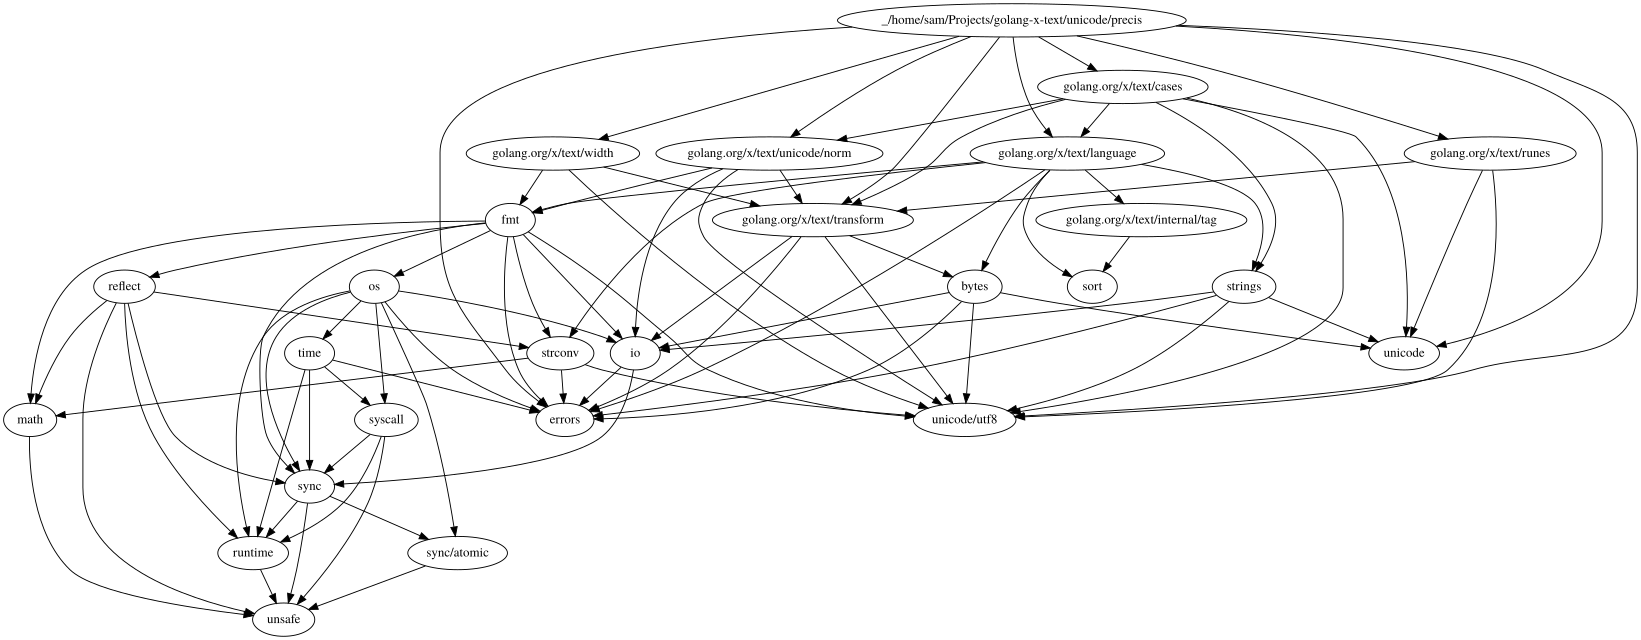
\includegraphics[width=\textwidth]{images/deps.svg.png}}
\end{frame}

\begin{frame}
	\frametitle{go vet}
	\begin{flushleft}
		Reports common mistakes such as:
	\end{flushleft}
	\begin{itemize}[<+(1)->]
		\item Format string/arg mismatch
		\item Variable shadowing
		\item Atomicity checks
		\item Unreachable code
		\item Long shifts (eg. someuint8 << 10)
		\item etc.
	\end{itemize}
\end{frame}

\begin{frame}
\frametitle{go tool}
\centerline{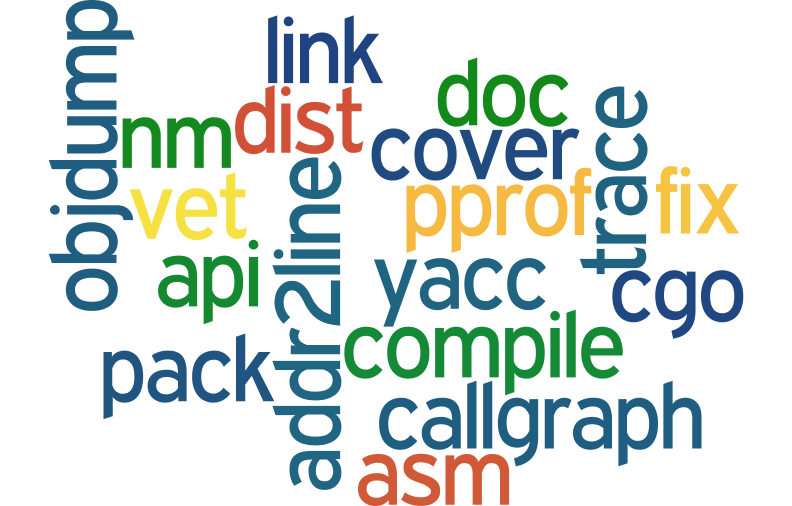
\includegraphics[width=0.75\textwidth]{images/tools.png}}
\end{frame}

\begin{frame}
	\frametitle{go test}
	\begin{flushleft}
		Go has a testing and benchmarking package built in.
	\end{flushleft}
	\begin{flushleft}
	\begin{itemize}[<+(1)->]
			\item Unit/integration testing
			\item Benchmarks
			\item Testable examples
			\item Helper package
			\begin{itemize}[<+(1)->]
				\item Failure logging
				\item Benchmark iteration
				\item etc.
			\end{itemize}
	\end{itemize}
	\end{flushleft}
\end{frame}

\begin{frame}
	\Large
	\begin{figure}
	{\color{AshGray}%
		\tikzmark{begin}sam\tikzmark{atsep}@%
		\tikzmark{domainpart}\textcolor{Cyan}{SamWhited}\tikzmark{tld}.com\tikzmark{end}%
	}

		\tikz[overlay,remember picture] {
			\draw[decorate,decoration={brace,raise=5mm,amplitude=15pt}] (begin.north
			west) -- node [above=1.75em] {\small email \& jid} (end.north east) ;
			\draw[decorate,decoration={brace,raise=2mm,amplitude=5pt,mirror}]
			(begin.south west) -- node[below of=begin, below=-1.35em] {\tiny me} (atsep.south west) ;
			\draw[decorate,decoration={brace,raise=2mm,amplitude=5pt,mirror}]
			(domainpart.south west) -- node[below of=begin, below=-1.35em] {\tiny twitter
			\addfontfeature{Variant=1}{\&} bitbucket } (tld.south west) ;
			\draw[decorate,decoration={brace,raise=6mm,amplitude=10pt,mirror}]
			(domainpart.south west) -- node[below of=begin, below=-.125em] {\tiny blog} (end.south west) ;
		}
	\end{figure}
\end{frame}

\end{document}
